\documentclass[11pt]{article}

\usepackage[a4paper,margin=0.92in]{geometry}
\usepackage[T1]{fontenc}
\usepackage[utf8]{inputenc}
\usepackage{lmodern}
\usepackage{microtype}
\usepackage{amsmath,amssymb,amsthm,mathtools}
\usepackage{booktabs,array}
\usepackage{enumitem}
\usepackage{xcolor}
\usepackage{tikz}
\usepackage[hidelinks]{hyperref}

\usetikzlibrary{arrows.meta,calc,positioning,shapes.geometric}

\hypersetup{
  pdftitle={Physical Analog Pandrosion for Continuous-Time Root Extraction},
  pdfauthor={Ivan Besevic},
  pdfsubject={Analog root extraction, translinear computation, Pandrosion, noise stability},
  pdfkeywords={Pandrosion, analog computation, translinear circuits, root extraction, finite-slope methods}
}
\setlength{\emergencystretch}{2em}

\newtheorem{definition}{Definition}[section]
\newtheorem{proposition}[definition]{Proposition}
\newtheorem{theorem}[definition]{Theorem}
\newtheorem{lemma}[definition]{Lemma}
\newtheorem{corollary}[definition]{Corollary}
\newtheorem{remark}[definition]{Remark}
\newtheorem{assumption}[definition]{Assumption}

\newcommand{\R}{\mathbb R}
\newcommand{\C}{\mathbb C}
\newcommand{\eps}{\varepsilon}
\newcommand{\dd}{\,\mathrm d}
\newcommand{\Sp}{S_p}
\newcommand{\hp}{h_{p,y}}
\newcommand{\OO}{\mathcal O}
\newcommand{\norm}[1]{\left\lVert #1\right\rVert}
\DeclareMathOperator{\Var}{Var}

\title{Physical Analog Pandrosion for Continuous-Time Root Extraction\\[3pt]
\large A corrected circuit-physics version of the legacy analog paper}
\author{Ivan Besevic\\Independent Mathematical Research}
\date{May 2026}

\begin{document}
\maketitle

\begin{abstract}
This paper rebuilds the legacy note \emph{Analog Pandrosion} as a physics-facing
research article.  The original note proposed a lookup-free and clockless
analog architecture for computing \(p\)-th roots from the monomial Pandrosion
map
\[
        h_{p,y}(s)=1-\frac{y-1}{y(1+s+\cdots+s^{p-1})}.
\]
The main correction is one of scope.  Analog root extraction is not new:
log-domain and computational-unit devices already implement products,
quotients, powers, and roots.  The contribution claimed here is narrower and
testable: Pandrosion gives a repeated, derivative-free, positive-domain
\(h\)-cell whose residual multiplier is controlled by the chart-normalized
target \(y\), and whose physical error can be bounded by the same
normalization and atlas principles developed in Papers 000--023.

We formulate a dimensionally consistent signal model, a positive-current
log/translinear implementation, and a voltage-mode macrocell implementation.
The chart selector from the monomial and atlas papers keeps \(y\ge 1\) and
\(|\log y|\) small, avoiding sign changes in the numerator and keeping the
denominator \(yS_p(s)\) away from zero.  For a normalized target satisfying
\(1\le y\le q^{p/(2K)}\), the fixed-point multiplier is bounded by
\[
        \Lambda_{p,q,K}=1-\frac{p}{S_p(q^{1/(2K)})}.
\]
This gives a direct small-signal stability estimate for deterministic
component offsets, thermal noise, multiplier gain error, divider error, and
finite settling.  A repeated \(h\)-cell pipeline is therefore not presented as
an operation-minimal replacement for digital Newton or for existing analog
computational units.  It is presented as a modular physical realization of the
Pandrosion geometry: a continuous-time normalized root cell whose accuracy is
set by chart normalization, component nonidealities, and settling bandwidth.
\end{abstract}

\paragraph{One-sentence summary.}
The improved analog claim is not ``first analog root circuit''; it is
``a positive-domain, chart-normalized, repeated Pandrosion \(h\)-cell with a
closed residual multiplier and explicit physical error budget.''

\paragraph{Status ledger.}
The fixed-point, chart-normalization, and multiplier bounds are mathematical
consequences of Papers 000--002 and 009--010.  The circuit models below are
architectural physics models, not a fabricated silicon result.  SPICE,
layout parasitics, temperature drift, and measured bandwidth remain required
before any hardware performance claim should be made.

\tableofcontents

\section{Why the legacy analog paper needs a rebuild}

The legacy April 2026 note made a strong claim: a Pandrosion pipeline computes
\(p\)-th roots with additions, multiplications, and division, without
derivatives, lookup tables, stored coefficients, or a clock.  That core idea is
worth preserving, but three statements need to be sharpened.

\begin{enumerate}[leftmargin=2em]
\item Analog root extraction already exists.  Classical log-domain,
translinear, and real-time computational-unit circuits can compute products,
quotients, powers, and roots.  The AD538, for example, is explicitly marketed
as a real-time analog computational unit with resistor-programmable powers and
roots.  Therefore the novelty cannot be ``analog root extraction exists''.
\item Operation count is not a sufficient physical metric.  A single
Pandrosion \(h\)-cell for \(p=3\) uses a polynomial ladder, a multiplier, a
divider, and a subtractor.  A useful pipeline repeats that cell.  The relevant
metrics are error budget, bandwidth, stability margin, dynamic range, offset,
temperature drift, and calibration complexity.
\item ``Clockless'' means continuous-time settling, not infinite-speed
computation.  A combinational analog chain has propagation delay, finite
bandwidth, parasitic poles, slew limits, and output settling error.  If the
result is consumed by a digital system, a sample-and-hold or ADC introduces a
clock at the interface.
\end{enumerate}

The improved claim is consequently narrower.  Pandrosion supplies a repeated
cell with one algebraic shape, no derivative block, no table lookup, and a
closed residual multiplier.  The physical question is whether this repeated
cell can be made accurate and stable enough, in the target bandwidth and power
range, to be useful.

\section{Inputs imported from Papers 000--023}

The present paper reads the current May 2026 series as the mathematical
backbone for a corrected physics paper.  The following table records what is
used from each article.

\begin{center}
\small
\begin{tabular}{@{}p{0.10\linewidth}p{0.82\linewidth}@{}}
\toprule
Paper & Role in the analog rebuild\\
\midrule
000 & Monomial Pandrosion map, fixed point, exact multiplier, Thales scaling, reciprocal chart, scale-palette theorem.\\
001 & Chart-scaled finite-slope solver ladder and the root-coordinate normalization \(u^p=y\).\\
002 & Divided-difference interpretation and fixed-anchor residual law.\\
003 & Chart optimization and local curvature cancellation.\\
004 & Higher-order jet cancellation and the inverse-chart principle.\\
005 & Tensorial multidimensional reading of finite-slope blocks.\\
006 & Equal-value pole geometry, relevant to avoiding divider singularities.\\
007 & Variational chart geometry and distributed flattening over a domain.\\
008 & Finite-slope descent and Lyapunov viewpoint for accepted corrections.\\
009 & Dynamic atlas language: chart scores, homothety, inversion, transition rules.\\
010 & Stable numerical atlases and projective conditioning.\\
011 & Probe paths and stability metrics.\\
012 & Low-action/geodesic interpretation of stable probes.\\
013 & Conditional geometric descent statements.\\
014 & All-order tensor inverse jets.\\
015 & Uniform finite atlas and anchor-palette logic.\\
016 & Analytic convergence under Lojasiewicz-type descent.\\
017 & Finite-probe reconstruction as a derivative-free physical measurement model.\\
018 & Equal-value pole monodromy and pole-collision caution.\\
019 & Discrete probe convergence, relevant to finite sampled hardware probes.\\
020 & Finite-slope polynomial-system framework and honest conditional status.\\
021 & Average-polynomial formulation and failure-probability amplification style.\\
022 & Universal atlas viewpoint and fixed-cell geometry.\\
023 & Hypercube design, random-matrix stabilization, and explicit proof ledger discipline.\\
\bottomrule
\end{tabular}
\end{center}

The analog paper uses only the monomial positive-real part as a proposed
hardware primitive.  The later atlas and finite-probe papers enter as design
discipline: normalize first, avoid equal-value poles, keep charts well
conditioned, and separate proved statements from experiments.

\section{Mathematical core of the root cell}

Let \(p\ge 2\) and \(y>0\).  Define
\[
        \Sp(s)=1+s+\cdots+s^{p-1},
        \qquad
        \hp(s)=1-\frac{y-1}{y\Sp(s)}.
\]
For \(y\ge1\), the positive fixed point is
\[
        s_*=y^{-1/p},
        \qquad
        u_*=y s_*^{p-1}=y^{1/p}.
\]
Thus \(s\) is the internal reciprocal-root coordinate and \(u\) is the visible
root-coordinate readout.

\begin{proposition}[Fixed point and readout]
For \(y>0\), \(s_*=y^{-1/p}\) is a fixed point of \(\hp\), and
\[
        y s_*^{p-1}=y^{1/p}.
\]
\end{proposition}

\begin{proof}
At \(s_*=y^{-1/p}\), one has
\[
        y\Sp(s_*)=\frac{y(1-s_*^p)}{1-s_*}
        =\frac{y-1}{1-s_*}
\]
when \(s_*\ne1\), with the case \(s_*=1\) obtained by continuity.  Hence
\[
        1-\frac{y-1}{y\Sp(s_*)}=s_*.
\]
The readout identity follows from \(s_*^p=1/y\).
\end{proof}

\begin{proposition}[Exact local multiplier]
Put \(\alpha=y^{1/p}\).  At the positive fixed point,
\[
        \lambda_{p,y}=\hp'(s_*)=
        1-\frac{p}{1+\alpha+\cdots+\alpha^{p-1}}.
\]
In particular, \(\lambda_{p,1}=0\), and \(\lambda_{p,y}\) grows as \(y\) moves
away from \(1\) on the branch \(y\ge1\).
\end{proposition}

This multiplier is the main reason an analog implementation should include a
chart/scale selector before the \(h\)-pipeline.  A raw circuit forced to handle
all magnitudes in one affine chart has a poor residual multiplier and a poor
physical dynamic range.

\section{Dimensional normalization and chart selection}

Physical voltages and currents have units.  The map \(\hp\) is dimensionless.
Therefore a root extractor must first convert the input signal to a
dimensionless normalized target.

Let \(X(t)>0\) be the physical input quantity and let \(B>0\) be a physical
root-scale, with units chosen so that \(B^p\) has the units of \(X\).  There
are two positive charts:
\[
        y_+(B)=\frac{X}{B^p},
        \qquad
        y_\infty(B)=\frac{B^p}{X}.
\]
The direct chart returns \(Z=B u\).  The reciprocal chart returns \(Z=B/u\).
Both are physically valid because
\[
        u^p=y_+(B)\Rightarrow (Bu)^p=X,
        \qquad
        u^p=y_\infty(B)\Rightarrow (B/u)^p=X.
\]

Choose a root-scale palette
\[
        \mathcal B_{q,K}=\{q^{m+j/K}B_0:m\in\mathbb Z,\;j=0,\ldots,K-1\}.
\]
The selector chooses a chart and scale such that \(y\ge1\) and \(\log y\) is
minimal.  The monomial scale-palette theorem gives
\[
        1\le y\le q^{p/(2K)},
        \qquad
        1\le y^{1/p}\le q^{1/(2K)}.
\]

\begin{theorem}[Normalized physical multiplier bound]
Assume the chart selector gives \(1\le y\le q^{p/(2K)}\).  Then the local
residual multiplier of the analog \(h\)-cell satisfies
\[
        0\le \lambda_{p,y}\le
        \Lambda_{p,q,K}:=
        1-\frac{p}{1+q^{1/(2K)}+\cdots+q^{(p-1)/(2K)}}.
\]
\end{theorem}

\begin{proof}
The multiplier formula depends monotonically on
\(\alpha=y^{1/p}\ge1\).  The selector gives
\(\alpha\le q^{1/(2K)}\).  Substitution gives the bound.
\end{proof}

This theorem is the hardware version of the chart-scaling message: the
physical cell should not be asked to compute roots over decades of input
range without first moving the problem into a bounded root-coordinate annulus.

\section{The \(h\)-cell as a physical block}

For a fixed normalized target \(y\ge1\), an \(h\)-cell maps an input \(s\) to
\[
        s^+=1-\frac{y-1}{y\Sp(s)}.
\]
The cell contains four conceptual subblocks:
\[
        s\mapsto \Sp(s),\qquad
        (y,\Sp)\mapsto y\Sp,\qquad
        (y-1,y\Sp)\mapsto \frac{y-1}{y\Sp},\qquad
        r\mapsto1-r.
\]
The numerator \(y-1\) is shared across repeated stages for a fixed input
sample or slowly varying input trajectory.  It should not be counted once per
stage in a physical layout unless each stage has its own independent input
conditioner.

\begin{figure}[htbp]
\centering
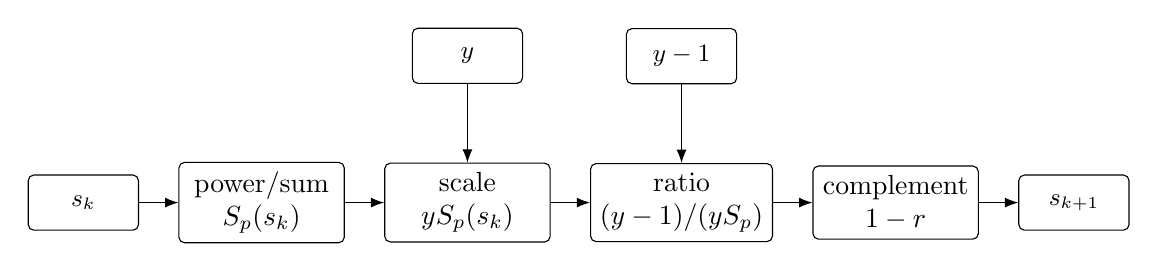
\begin{tikzpicture}[
  block/.style={draw,rounded corners=2pt,minimum height=9mm,minimum width=21mm,align=center},
  tinyblock/.style={draw,rounded corners=2pt,minimum height=7mm,minimum width=14mm,align=center,font=\small},
  >=Latex
]
\node[tinyblock] (s) {\(s_k\)};
\node[block,right=5mm of s] (poly) {power/sum\\\(\Sp(s_k)\)};
\node[block,right=5mm of poly] (mul) {scale\\\(y\Sp(s_k)\)};
\node[block,right=5mm of mul] (div) {ratio\\\((y-1)/(y\Sp)\)};
\node[block,right=5mm of div] (sub) {complement\\\(1-r\)};
\node[tinyblock,right=5mm of sub] (out) {\(s_{k+1}\)};
\node[tinyblock,above=10mm of mul] (y) {\(y\)};
\node[tinyblock,above=10mm of div] (num) {\(y-1\)};
\draw[->] (s) -- (poly);
\draw[->] (poly) -- (mul);
\draw[->] (mul) -- (div);
\draw[->] (div) -- (sub);
\draw[->] (sub) -- (out);
\draw[->] (y) -- (mul);
\draw[->] (num) -- (div);
\end{tikzpicture}
\caption{One normalized Pandrosion \(h\)-cell.  Repeated pipelines copy this
cell while sharing the normalized input \(y\) and numerator \(y-1\).}
\label{fig:hcell}
\end{figure}

\subsection{Current-mode log/translinear realization}

The cleanest physics model uses positive currents.  Encode each positive
dimensionless variable \(a\) by a current \(I_a=I_0a\), or in a log-domain
variant by a voltage \(V_a=U_T\log a\) where \(U_T=kT/q_e\).  Sums are natural
in current mode:
\[
        I_{\Sp}=I_0+I_s+I_{s^2}+\cdots+I_{s^{p-1}}.
\]
Products and quotients can be formed by translinear loops or log/antilog
blocks:
\[
        I_{ab}=\frac{I_aI_b}{I_0},
        \qquad
        I_{a/b}=\frac{I_aI_0}{I_b}.
\]
The Pandrosion denominator is strictly positive:
\[
        I_{y\Sp}\ge I_y>0,
\]
so the divider is not exposed to the equal-value pole inside the intended
positive chart.

\begin{remark}[Temperature]
Log-domain circuits inherit explicit thermal-voltage dependence.  A raw
implementation is therefore temperature sensitive.  A credible design must use
matched devices, ratioed currents, bias tracking, or calibration.  The
Pandrosion geometry removes derivative and lookup blocks; it does not remove
semiconductor physics.
\end{remark}

\subsection{Voltage-mode macrocell realization}

For a board-level demonstrator, the same block can be built from analog
multipliers, op-amp summers, and a divider.  Devices such as AD633 and AD835
are representative multiplier macrocells; AD538 is a representative analog
computational unit that already exposes powers and roots.  This matters for
positioning: a Pandrosion board should be compared against existing analog
computational units, not only against digital Newton.

For \(p=3\), a shared-input \(h\)-pipeline uses per cell:
\[
        s^2,\quad 1+s+s^2,\quad y(1+s+s^2),\quad
        \frac{y-1}{y(1+s+s^2)},\quad
        1-\frac{y-1}{y(1+s+s^2)}.
\]
The readout uses \(u=y s_N^2\), followed by \(Z=Bu\) in the direct chart or
\(Z=B/u\) in the reciprocal chart.

\section{Noise, offset, and settling model}

Let the physical cell be modeled as
\[
        \widetilde h(s)=h_{p,y}(s)+\beta(s,y)+\xi(s,y),
\]
where \(\beta\) is a deterministic bias term caused by gain error, offset,
nonlinearity, and finite settling, while \(\xi\) is zero-mean random noise.
Near the fixed point,
\[
        e_{k+1}=\lambda_{p,y}e_k+\beta_*+\xi_k+\OO(e_k^2),
        \qquad e_k=s_k-s_*.
\]

\begin{assumption}[Lumped cell error]
In the operating annulus selected by the chart layer, suppose
\[
        |\beta(s,y)|\le \beta_{\rm cell},
        \qquad
        \Var(\xi(s,y))\le \sigma_{\rm cell}^2,
        \qquad
        |\hp'(s)|\le \Lambda<1.
\]
\end{assumption}

\begin{theorem}[Pipeline error budget]
Under the lumped cell assumption, the \(N\)-cell pipeline satisfies, to first
order in the cell errors,
\[
        |\mathbb E e_N|
        \le
        \Lambda^N|e_0|+\frac{1-\Lambda^N}{1-\Lambda}\beta_{\rm cell},
\]
and, for independent stage noise,
\[
        \Var(e_N)
        \le
        \frac{1-\Lambda^{2N}}{1-\Lambda^2}\sigma_{\rm cell}^2.
\]
\end{theorem}

\begin{proof}
Iterate the affine stochastic recurrence
\[
        e_{k+1}=\Lambda e_k+\beta_k+\xi_k
\]
with \(|\beta_k|\le\beta_{\rm cell}\).  The expectation is bounded by a
geometric series.  Independence and zero mean give the variance series.
\end{proof}

\begin{corollary}[Why normalization is a physical requirement]
If the selector makes \(\Lambda=\Lambda_{p,q,K}\ll1\), both the deterministic
initial residual and the accumulated physical errors are suppressed by short
geometric sums.  If \(y\) is not normalized and \(\Lambda\approx1\), offsets,
thermal noise, and settling error accumulate almost linearly with pipeline
depth.
\end{corollary}

The legacy paper emphasized mathematical bias.  The corrected physical version
separates three different floors:
\[
        \text{math residual}+\text{deterministic circuit bias}
        +\text{random noise}.
\]
Post-filtering can reduce random noise but cannot remove a deterministic
mathematical residual or a systematic circuit offset.

\section{Deterministic bias of the normalized \(h\)-pipeline}

The following table gives exact floating-point evaluations of the ideal
mathematical \(h\)-pipeline for \(y=2\), initialized by the physical
preconditioning stage \(s_0=h_{p,2}(1)\).  The visible output is
\(u_N=y s_N^{p-1}\), and the error is \(|u_N-2^{1/p}|\).

\begin{center}
\small
\begin{tabular}{@{}ccccc@{}}
\toprule
\(p\) & stages \(1\) & stages \(2\) & stages \(3\) & stages \(4\)\\
\midrule
2 & \(8.58\cdot10^{-2}\) & \(1.44\cdot10^{-2}\) & \(2.45\cdot10^{-3}\) & \(4.21\cdot10^{-4}\)\\
3 & \(1.29\cdot10^{-1}\) & \(2.71\cdot10^{-2}\) & \(5.91\cdot10^{-3}\) & \(1.30\cdot10^{-3}\)\\
5 & \(1.64\cdot10^{-1}\) & \(3.93\cdot10^{-2}\) & \(9.92\cdot10^{-3}\) & \(2.53\cdot10^{-3}\)\\
\bottomrule
\end{tabular}
\end{center}

These numbers should not be read as a hardware benchmark.  They are a
deterministic residual table for the ideal map.  A real circuit adds the
offset/noise/settling budget of the previous section.  The table is useful
because it tells the circuit designer how much mathematical residual remains
before component physics is added.

\section{Comparison with Newton and analog computational units}

Newton's method for \(u^p=y\) uses
\[
        u^+=u-\frac{u^p-y}{p u^{p-1}}.
\]
It has excellent mathematical convergence when supplied with a good seed, but
the hardware block contains explicit \(p\)-dependent gain and a derivative
denominator.  In a digital processor this is not a problem; in a fixed analog
cell it changes the calibration surface.

The Pandrosion \(h\)-cell instead places the \(p\)-dependence in the polynomial
ladder \(S_p\).  This is not automatically cheaper.  It is a different
physical trade:
\[
\begin{array}{ll}
\text{Newton:} & \text{fewer iterations, derivative/gain-specific cell, seed sensitive;}\\
\text{Pandrosion:} & \text{repeated identical cells, derivative-free, chart-normalized.}
\end{array}
\]

Existing analog computational units provide another comparison class.  An
AD538-style part can directly implement powers and roots through a calibrated
log-domain computation.  A Pandrosion implementation must therefore justify
itself through modularity, absence of a stored table/seed, positive-domain
stability, or application-specific integration into a larger analog signal
path.  It should not claim to beat a mature computational unit without
measured data.

\section{Applications where the architecture is plausible}

\subsection{Sensor front-ends}

Low-power sensor front-ends often need monotone linearization, normalization,
or square-root-like compression before digitization.  A normalized
Pandrosion block could be useful when modest precision is enough and the root
operation is embedded in a continuous signal path.

\subsection{Radar and sonar magnitude channels}

Magnitude extraction involves operations such as
\[
        |z|=\sqrt{I^2+Q^2}.
\]
For \(p=2\), the polynomial ladder is shortest and the positive-domain
implementation is most attractive.  The actual performance question is whether
the multiplier/divider bandwidth and settling error beat a conventional
rectifier/RMS/computational-unit solution for the target frequency band.

\subsection{Neuromorphic and analog ML blocks}

Analog neuromorphic circuits often tolerate low to moderate precision but care
about locality, bandwidth, and power.  Power-law activations, normalization
terms, and \(L_p\)-norm approximations are plausible use cases.  The main
advantage would be keeping the operation inside the analog substrate rather
than converting to a digital processor for a single nonlinear function.

\section{Experimental program}

A defensible physics paper needs experiments in the following order.

\begin{enumerate}[leftmargin=2em]
\item \textbf{Behavioral SPICE.}  Implement ideal controlled-source \(h\)-cells
with finite bandwidth, offset, and noise.  Verify the multiplier-bound error
budget.
\item \textbf{Macrocell board.}  Build \(p=2\) and \(p=3\) boards using
commercial multipliers/dividers or log-ratio blocks.  Measure static transfer,
settling time, temperature drift, and output noise.
\item \textbf{Chart selector.}  Test direct and reciprocal normalization over
multiple decades of \(X\).  Verify that the root-coordinate output stays in the
predicted annulus.
\item \textbf{Comparison.}  Compare against a direct computational-unit root
circuit, a Newton-like analog macrocell, and a digital microcontroller baseline
at equal bandwidth and power.
\item \textbf{ASIC feasibility.}  Replace board-level macrocells by matched
translinear/log-domain cells and estimate area, power, calibration overhead,
and thermal sensitivity.
\end{enumerate}

\section{Falsifiable claims}

The improved analog program should be judged by the following falsifiable
claims.

\begin{enumerate}[leftmargin=2em]
\item With chart normalization, the measured small-signal residual factor of
the \(h\)-pipeline tracks the theoretical bound
\(\Lambda_{p,q,K}\) within the measured component error budget.
\item Repeating identical \(h\)-cells gives predictable deterministic residual
reduction until circuit offset or noise dominates.
\item The positive-domain denominator \(yS_p(s)\) prevents internal divider
singularities over the selected operating annulus.
\item For at least one target application, the complete analog block has a
power-latency-precision point that is competitive with direct analog
computational units or digitize-and-compute baselines.
\end{enumerate}

The first three claims are near-term circuit-physics checks.  The fourth is an
application-level engineering claim and should not be asserted without
measurements.

\section{Conclusion}

The legacy analog Pandrosion note contained a useful idea but overstated its
hardware novelty.  This rebuilt version gives the sharper claim.  Pandrosion
does not invent analog root extraction.  It supplies a derivative-free,
positive-domain, chart-normalized \(h\)-cell whose residual multiplier is known
exactly and whose physical errors admit a simple pipeline budget.  The right
next step is not another operation-count table; it is a measured \(p=2\) or
\(p=3\) demonstrator with explicit bandwidth, offset, noise, drift, and
comparison baselines.

\begin{thebibliography}{99}

\bibitem{Besevic000}
I. Besevic, \emph{A Monomial Pandrosion Scheme: Contraction, Chart Scaling,
and Steffensen Acceleration for \(z^p=x\)}, preprint, May 2026.

\bibitem{Besevic001}
I. Besevic, \emph{Chart-Scaled Cubic Pandrosion by Finite-Slope Halley
Acceleration}, preprint, May 2026.

\bibitem{Besevic002}
I. Besevic, \emph{Anchored Pandrosion for General Analytic Equations},
preprint, May 2026.

\bibitem{BesevicAtlas}
I. Besevic, \emph{Pandrosion Atlases and Dynamic Geometric Charts}, preprint,
May 2026.

\bibitem{BesevicStableAtlas}
I. Besevic, \emph{Stable Numerical Atlases for Pandrosion Dynamics}, preprint,
May 2026.

\bibitem{BesevicLegacyAnalog}
I. Besevic, \emph{Analog Pandrosion: A lookup-free, clockless circuit
architecture for \(p\)-th root extraction}, legacy preprint, April 2026.

\bibitem{AD633}
Analog Devices, \emph{AD633: Low Cost Analog Multiplier Data Sheet},
Rev. K, 2002.
\url{https://www.analog.com/en/products/ad633.html}

\bibitem{AD835}
Analog Devices, \emph{AD835: 250 MHz, Voltage Output 4-Quadrant Multiplier
Data Sheet}, Rev. E, 2010.
\url{https://www.analog.com/en/products/ad835.html}

\bibitem{AD538}
Analog Devices, \emph{AD538: Real-Time Analog Computational Unit Data Sheet},
Rev. E, 2006.
\url{https://www.analog.com/en/products/ad538.html}

\bibitem{Volder}
J. E. Volder, ``The CORDIC trigonometric computing technique,''
\emph{IRE Transactions on Electronic Computers}, EC-8(3), 330--334, 1959.

\bibitem{Muller}
J.-M. Muller, \emph{Elementary Functions: Algorithms and Implementation},
3rd ed., Birkhauser, 2016.

\bibitem{Markstein}
P. Markstein, \emph{IA-64 and Elementary Functions: Speed and Precision},
Prentice Hall, 2000.

\bibitem{Schuman}
C. D. Schuman et al., ``A survey of neuromorphic computing and neural
networks in hardware,'' arXiv:1705.06963, 2017.

\bibitem{Gilbert}
B. Gilbert, ``A precise four-quadrant multiplier with subnanosecond response,''
\emph{IEEE Journal of Solid-State Circuits}, 3(4), 365--373, 1968.

\end{thebibliography}

\end{document}
